% #############################################################################
% This is Chapter 2
% !TEX root = ../main.tex
% #############################################################################
% Change the Name of the Chapter i the following line
\fancychapter{Fundamental Concepts}
\cleardoublepage
% The following line allows to ref this chapter
\label{chap:back}

This chapter introduces the fundamental technical concepts and architectures underlying open-vocabulary referring segmentation systems. We begin with neural networks and deep learning fundamentals (Section~2.1), then review attention and the transformer architecture (Section~2.2). We next summarize how transformers have been adapted for computer vision (Section~2.3), followed by image segmentation variants (Section~2.4) and vision-language foundations relevant to referring segmentation (Section~2.5).

% #############################################################################
\section{Neural Networks and Deep Learning}

Neural networks form the foundation of modern deep learning systems, providing the computational framework for learning complex patterns from data. The perceptron represents the simplest form of artificial neural network, consisting of a single computational unit that performs a linear combination of inputs followed by a nonlinear activation function, as illustrated in Figure~\ref{fig:perceptron}. For a perceptron with $N$ input features $\mathbf{x} = [x_1, x_2, \ldots, x_N]^T$, the output $y$ is computed as:

\begin{equation}
y = f(\mathbf{w}^T\mathbf{x} + b),
\end{equation}

where $\mathbf{w} = [w_1, w_2, \ldots, w_N]^T$ represents the weight vector, $b$ is the bias term, and $f(\cdot)$ denotes the activation function. This can be expanded as:

\begin{equation}
y = f\left(\sum_{i=1}^{N} w_i x_i + b\right).
\end{equation}

The activation function $f(\cdot)$ introduces nonlinearity into the model, enabling the perceptron to learn complex decision boundaries. Common activation functions include the sigmoid function $f(z) = \frac{1}{1 + e^{-z}}$, the hyperbolic tangent $f(z) = \tanh(z)$, and the rectified linear unit (ReLU) $f(z) = \max(0, z)$.

Multi-layer perceptrons extend the single perceptron by connecting multiple layers of neurons in a feedforward architecture, as shown in Figure~\ref{fig:mlp}. For a neural network with $L$ layers, where layer $l$ contains $n_l$ neurons, the forward propagation process computes:

\begin{equation}
\mathbf{a}^{(l)} = f^{(l)}\left(\mathbf{W}^{(l)}\mathbf{a}^{(l-1)} + \mathbf{b}^{(l)}\right),
\end{equation}

where $\mathbf{a}^{(l)}$ represents the activation vector of layer $l$, $\mathbf{W}^{(l)} \in \mathbb{R}^{n_l \times n_{l-1}}$ is the weight matrix connecting layers $l-1$ and $l$, $\mathbf{b}^{(l)} \in \mathbb{R}^{n_l}$ is the bias vector, and $f^{(l)}(\cdot)$ is the activation function for layer $l$. The universal approximation theorem demonstrates that multi-layer perceptrons with sufficient hidden units can approximate any continuous function on compact subsets of $\mathbb{R}^n$, providing the theoretical foundation for their expressiveness.

Neural networks are trained through gradient-based optimization methods that minimize a loss function $\mathcal{L}(\theta)$, where $\theta$ represents all learnable parameters. The loss function quantifies the difference between predicted outputs and ground truth targets, such as the mean squared error for regression tasks:

\begin{equation}
\mathcal{L}(\theta) = \frac{1}{n}\sum_{i=1}^{n}(y_i - \hat{y}_i)^2,
\end{equation}

where $n$ is the number of training samples, $y_i$ are the true labels, and $\hat{y}_i$ are the predicted outputs. The backpropagation algorithm efficiently computes gradients by applying the chain rule of calculus. The most common optimization algorithm is stochastic gradient descent, which updates parameters according to:

\begin{equation}
\theta_{t+1} = \theta_t - \eta \nabla_\theta \mathcal{L}(\theta_t),
\end{equation}

where $\eta$ is the learning rate and $\nabla_\theta \mathcal{L}(\theta_t)$ represents the gradient of the loss function with respect to parameters at iteration $t$.

\begin{figure}[t]
\centering
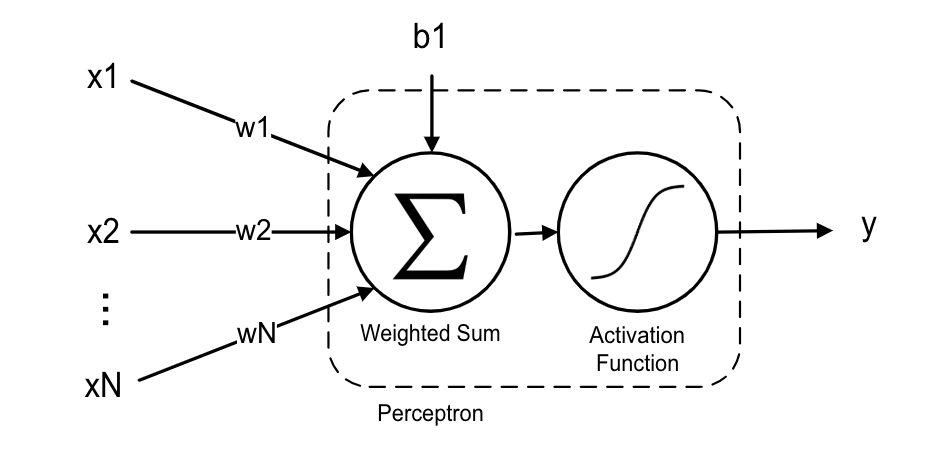
\includegraphics[width=0.6\textwidth]{Images/perceptron.png}
\caption{Perceptron architecture and basic neural network building block with inputs $x_1, x_2, \ldots, x_N$ and weights $w_1, \ldots, w_N$.}
\label{fig:perceptron}
\end{figure}

\begin{figure}[t]
\centering
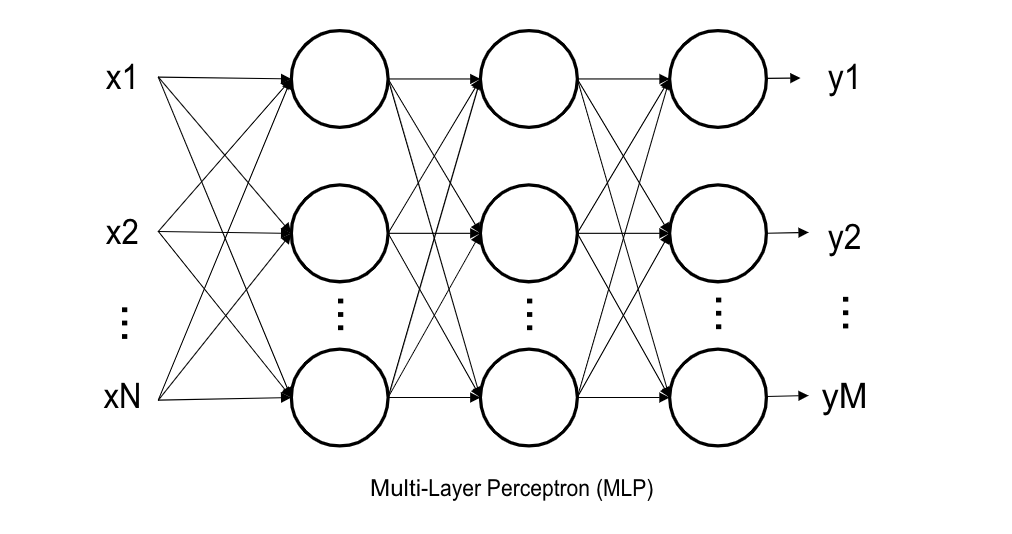
\includegraphics[width=0.6\textwidth]{Images/mlp.png}
\caption{Multi-layer perceptron architecture showing feedforward neural network structure operating on feature inputs $x_1, x_2, \ldots, x_N$.}
\label{fig:mlp}
\end{figure}

% #############################################################################
\section{Attention and Transformers}

The transformer architecture revolutionized sequence modeling by introducing a self-attention mechanism that enables models to process variable-length sequences more effectively than traditional fixed-size approaches. Unlike multi-layer perceptrons that operate on fixed-dimensional inputs, transformers can handle sequences of arbitrary length and are particularly effective at capturing long-range dependencies in medium to long sequences through the self-attention mechanism, making them suitable for tasks across multiple modalities including natural language, vision, audio, time series, or any sequential data where relationships between distant elements are important.

The core innovation of transformers lies in the self-attention mechanism, which allows each element in a sequence to attend to all other elements simultaneously, as illustrated in Figure~\ref{fig:transformer}. For a sequence of input tokens represented as embeddings $\mathbf{X} = [\mathbf{x}_1, \mathbf{x}_2, \ldots, \mathbf{x}_n] \in \mathbb{R}^{n \times d}$, where $n$ is the sequence length and $d$ is the embedding dimension, the self-attention mechanism computes three matrices: queries ($\mathbf{Q}$), keys ($\mathbf{K}$), and values ($\mathbf{V}$):

\begin{equation}
\mathbf{Q} = \mathbf{X}\mathbf{W}_Q, \quad \mathbf{K} = \mathbf{X}\mathbf{W}_K, \quad \mathbf{V} = \mathbf{X}\mathbf{W}_V,
\end{equation}

where $\mathbf{W}_Q, \mathbf{W}_K, \mathbf{W}_V \in \mathbb{R}^{d \times d_k}$ are learned parameter matrices. The attention scores $\boldsymbol{\alpha}$ are computed as:

\begin{equation}
\boldsymbol{\alpha} = \text{softmax}\left(\frac{\mathbf{Q}\mathbf{K}^T}{\sqrt{d_k}}\right),
\end{equation}

where the scaling factor $\sqrt{d_k}$ prevents the softmax function from saturating for large embedding dimensions. The final attention output is then computed as:

\begin{equation}
\text{Attention}(\mathbf{Q}, \mathbf{K}, \mathbf{V}) = \boldsymbol{\alpha}\mathbf{V},
\end{equation}

where $\boldsymbol{\alpha}$ represents the attention weights that determine how much each value $\mathbf{V}$ contributes to the output.

Since transformers process all positions in parallel, they lack inherent positional information. To address this, positional encodings are added to input embeddings to provide the model with information about token positions. The original transformer uses sinusoidal positional encodings:

\begin{equation}
PE_{(pos, 2i)} = \sin\left(\frac{pos}{10000^{2i/d}}\right), \quad PE_{(pos, 2i+1)} = \cos\left(\frac{pos}{10000^{2i/d}}\right),
\end{equation}

where $pos$ is the position index and $i$ is the dimension index. This encoding scheme allows the model to learn relative positions and generalizes to sequences longer than those seen during training.

The transformer block combines self-attention with feed-forward layers and residual connections. Each block applies layer normalization before both the attention and feed-forward operations, following the pre-normalization variant. The complete transformation for a single transformer block can be expressed as:

\begin{equation}
\mathbf{H}' = \text{Attention}(\text{LayerNorm}(\mathbf{H})) + \mathbf{H},
\end{equation}

\begin{equation}
\mathbf{H}'' = \text{FFN}(\text{LayerNorm}(\mathbf{H}')) + \mathbf{H}',
\end{equation}

where $\mathbf{H}$ represents the input hidden states and FFN denotes the feed-forward network. Multiple transformer blocks can be stacked to create deeper models that capture increasingly complex patterns in the input sequences. The output token embeddings from the final transformer layer can then be used for downstream tasks by attaching task-specific heads, such as classification layers for sentiment analysis or language modeling heads for text generation.

\begin{figure}[t]
\centering
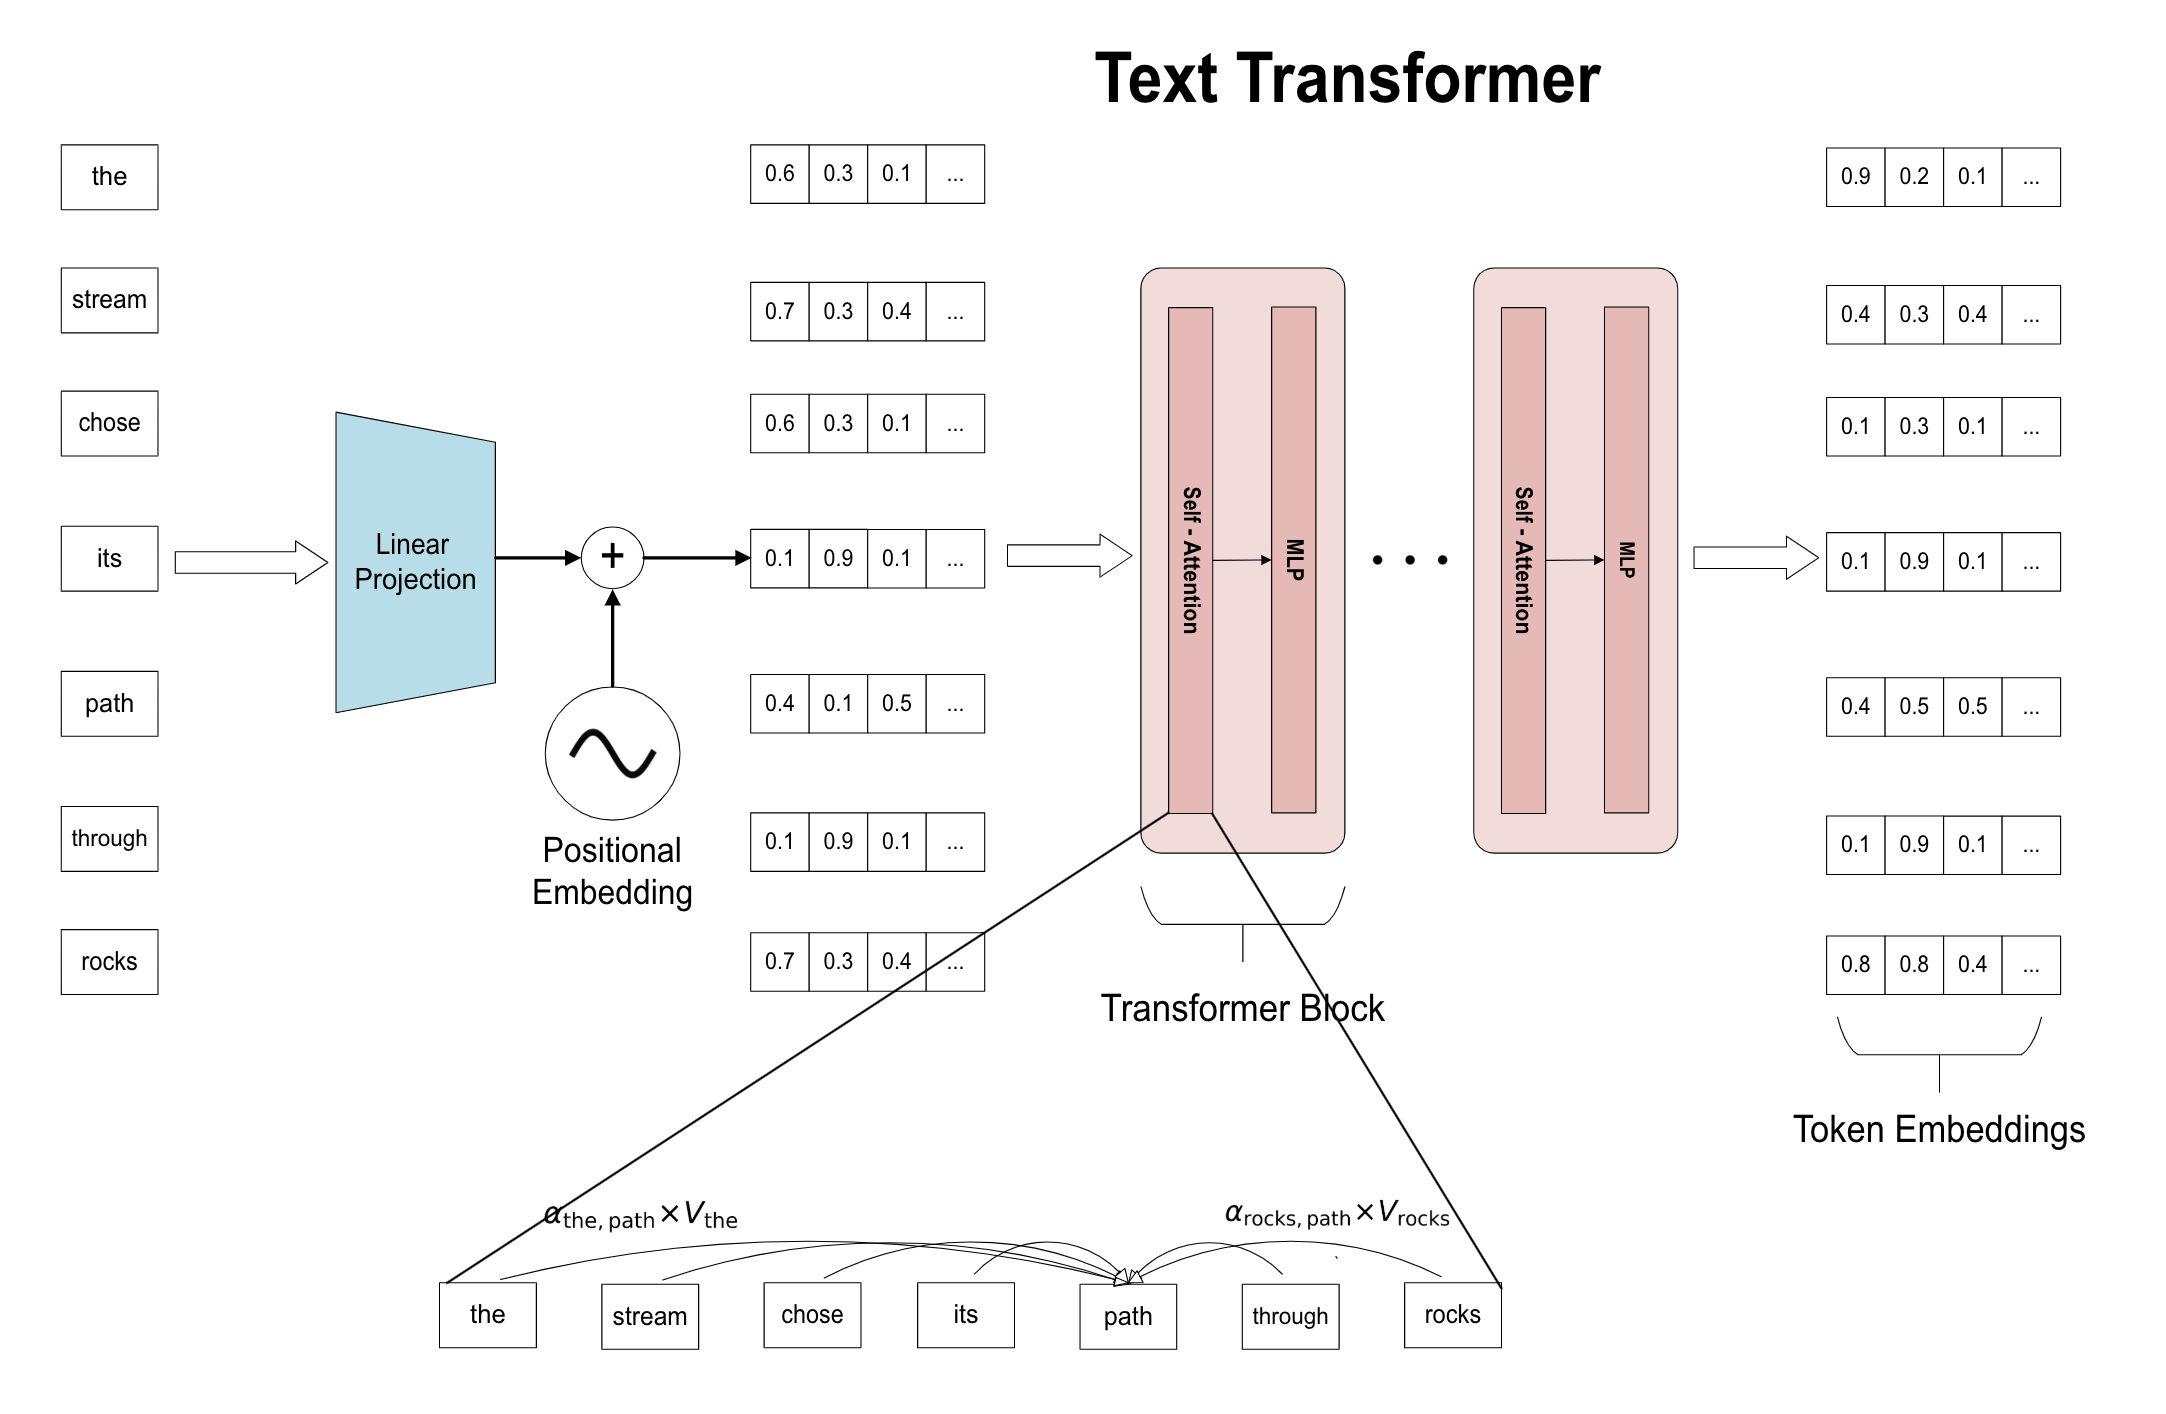
\includegraphics[width=0.9\textwidth]{Images/transformer.png}
\caption{Self-attention mechanism in transformers. The diagram shows how attention scores $\alpha$ are computed for each token, with specific examples of attention weights for tokens "path" and "rocks" relative to other words in the sequence "the stream chose its path through rocks".}
\label{fig:transformer}
\end{figure}

% #############################################################################
\section{Transformers for Computer Vision}

The success of transformers in natural language processing led to their adaptation for computer vision tasks, demonstrating the versatility of the self-attention mechanism across different modalities. Vision Transformers (ViTs) extend the transformer architecture to images by treating image patches as sequences of tokens, similar to how text transformers process word sequences.

The Vision Transformer architecture begins by dividing an input image into fixed-size square patches, as illustrated in Figure~\ref{fig:vit}. For an image of size $H \times W \times C$, where $H$ and $W$ are the height and width, and $C$ is the number of channels, the image is divided into $N = \frac{HW}{P^2}$ patches of size $P \times P$. Each patch is then flattened and linearly projected to create patch embeddings:

\begin{equation}
\mathbf{x}_p^{(i)} = \text{Linear}(\text{Flatten}(\mathbf{I}_p^{(i)})),
\end{equation}

where $\mathbf{I}_p^{(i)}$ represents the $i$-th patch and $\mathbf{x}_p^{(i)} \in \mathbb{R}^D$ is the corresponding patch embedding with dimension $D$.

Similar to text transformers, positional embeddings are added to patch embeddings to preserve spatial information about the patch locations within the original image. The sequence of patch embeddings is then processed through standard transformer blocks, applying self-attention mechanisms to capture relationships between different spatial regions of the image. This approach allows the model to learn which parts of the image are most relevant for the given task, whether it be classification, object detection, or feature extraction.

The output patch embeddings from the final transformer layer provide rich spatial representations that can be utilized for various computer vision tasks by attaching appropriate task-specific heads, such as classification heads for image categorization or detection heads for object localization. The Vision Transformer demonstrates that the same architectural principles underlying text transformers can be successfully applied to visual data, reinforcing the universal applicability of self-attention mechanisms across multiple modalities including text, vision, and other sequential data types.

\begin{figure}[t]
\centering
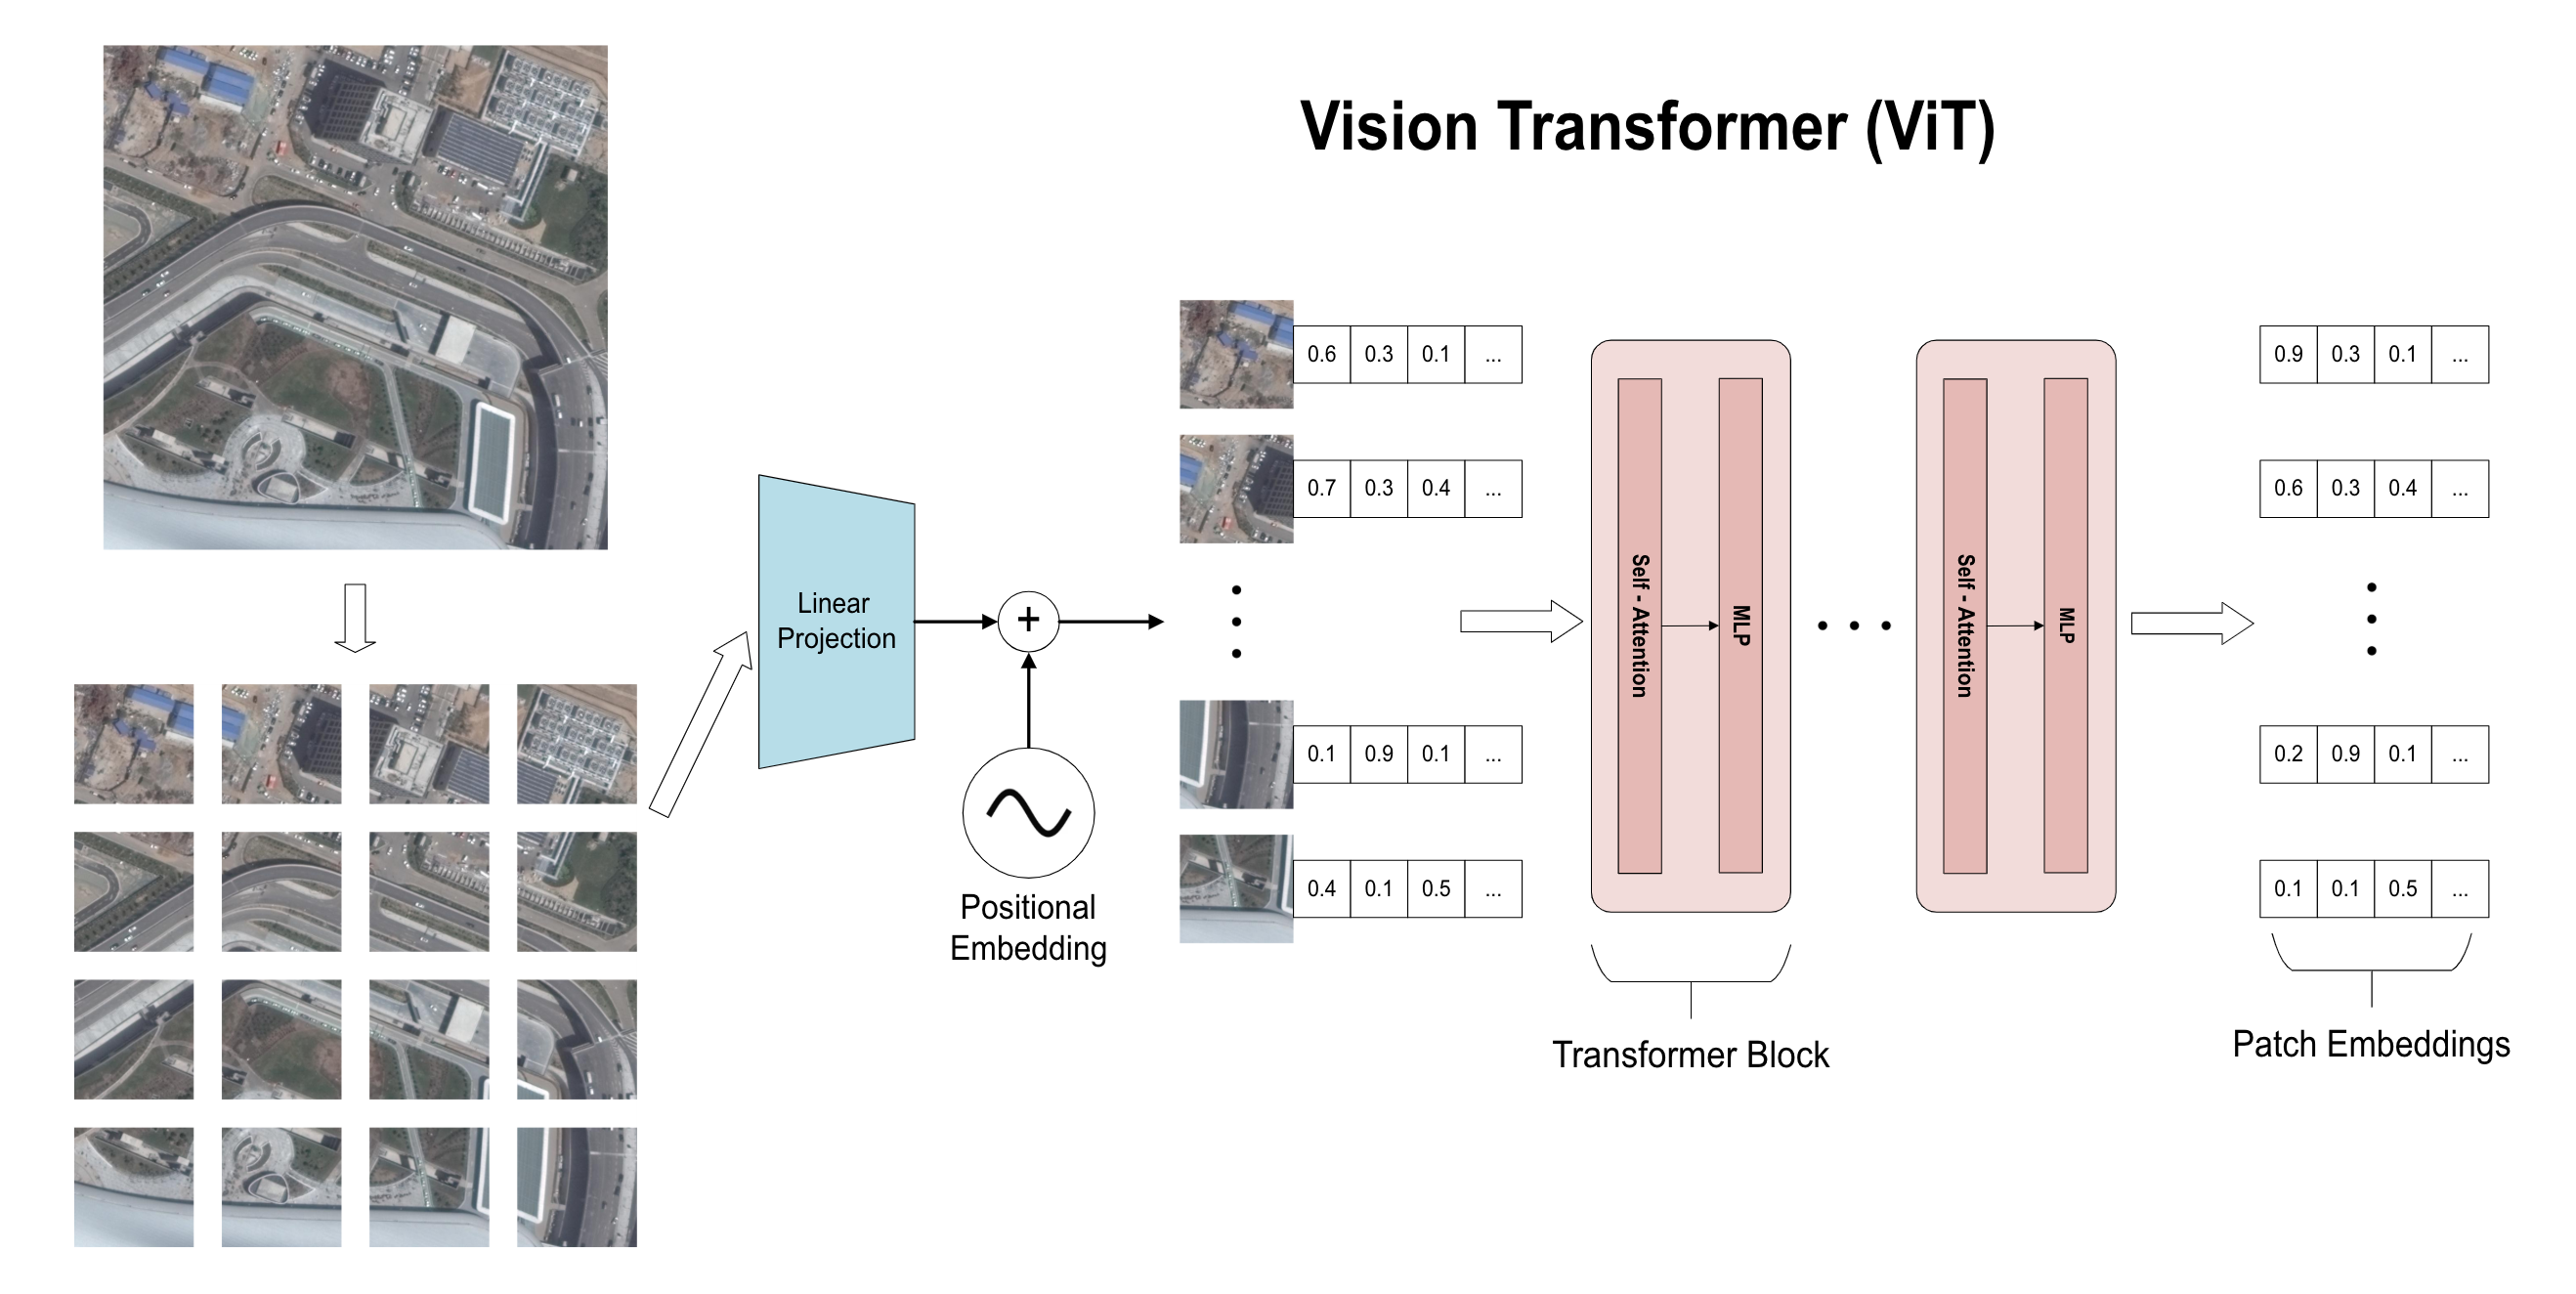
\includegraphics[width=0.9\textwidth]{Images/vit.png}
\caption{Vision Transformer (ViT) architecture for image classification and feature extraction. The input image is divided into square patches, which are then linearly projected and processed through transformer blocks, similar to how text transformers handle word tokens.}
\label{fig:vit}
\end{figure}


% #############################################################################
\section{Image Segmentation}

Image segmentation is a fundamental computer vision task that involves partitioning an image into semantically meaningful regions by classifying each pixel according to its content. At its core, segmentation can be viewed as a dense prediction problem where the model performs pixel-level binary or multi-class classification, determining for each spatial location whether it belongs to a particular object or region of interest.

The segmentation process transforms an input image $\mathbf{I} \in \mathbb{R}^{H \times W \times C}$ into a segmentation mask $\mathbf{M} \in \{0, 1\}^{H \times W}$ for binary segmentation, or $\mathbf{M} \in \{0, 1, \ldots, K\}^{H \times W}$ for multi-class segmentation with $K$ categories. Each pixel $(i, j)$ in the output mask $\mathbf{M}_{i,j}$ represents the predicted class label for the corresponding spatial location in the input image.

Different variations of the segmentation task address distinct aspects of scene understanding, as illustrated in Figure~\ref{fig:segmentation}. Semantic segmentation assigns each pixel to a predefined semantic category, such as "small vehicle," "large vehicle," or "plane," without distinguishing between individual object instances within the same category. This approach provides a comprehensive understanding of scene composition but treats all objects of the same class as a single entity.

Instance segmentation extends semantic segmentation by identifying and delineating individual object instances, enabling the model to distinguish between separate objects that belong to the same semantic category. For example, multiple aircraft in an aerial image would be segmented as distinct entities rather than merged into a single "plane" region. This capability is crucial for applications requiring precise object counting and individual object analysis.

Referring instance segmentation represents the most sophisticated variant, combining instance-level precision with natural language understanding. This task requires the model to segment a specific object instance based on a natural language description or prompt, such as "large vehicle in between two planes." The model must simultaneously understand the linguistic description and identify the corresponding visual region, bridging the gap between language and vision modalities. This approach enables more intuitive human-computer interaction and supports complex queries that cannot be addressed through traditional category-based segmentation methods.

\begin{figure}[t]
\centering
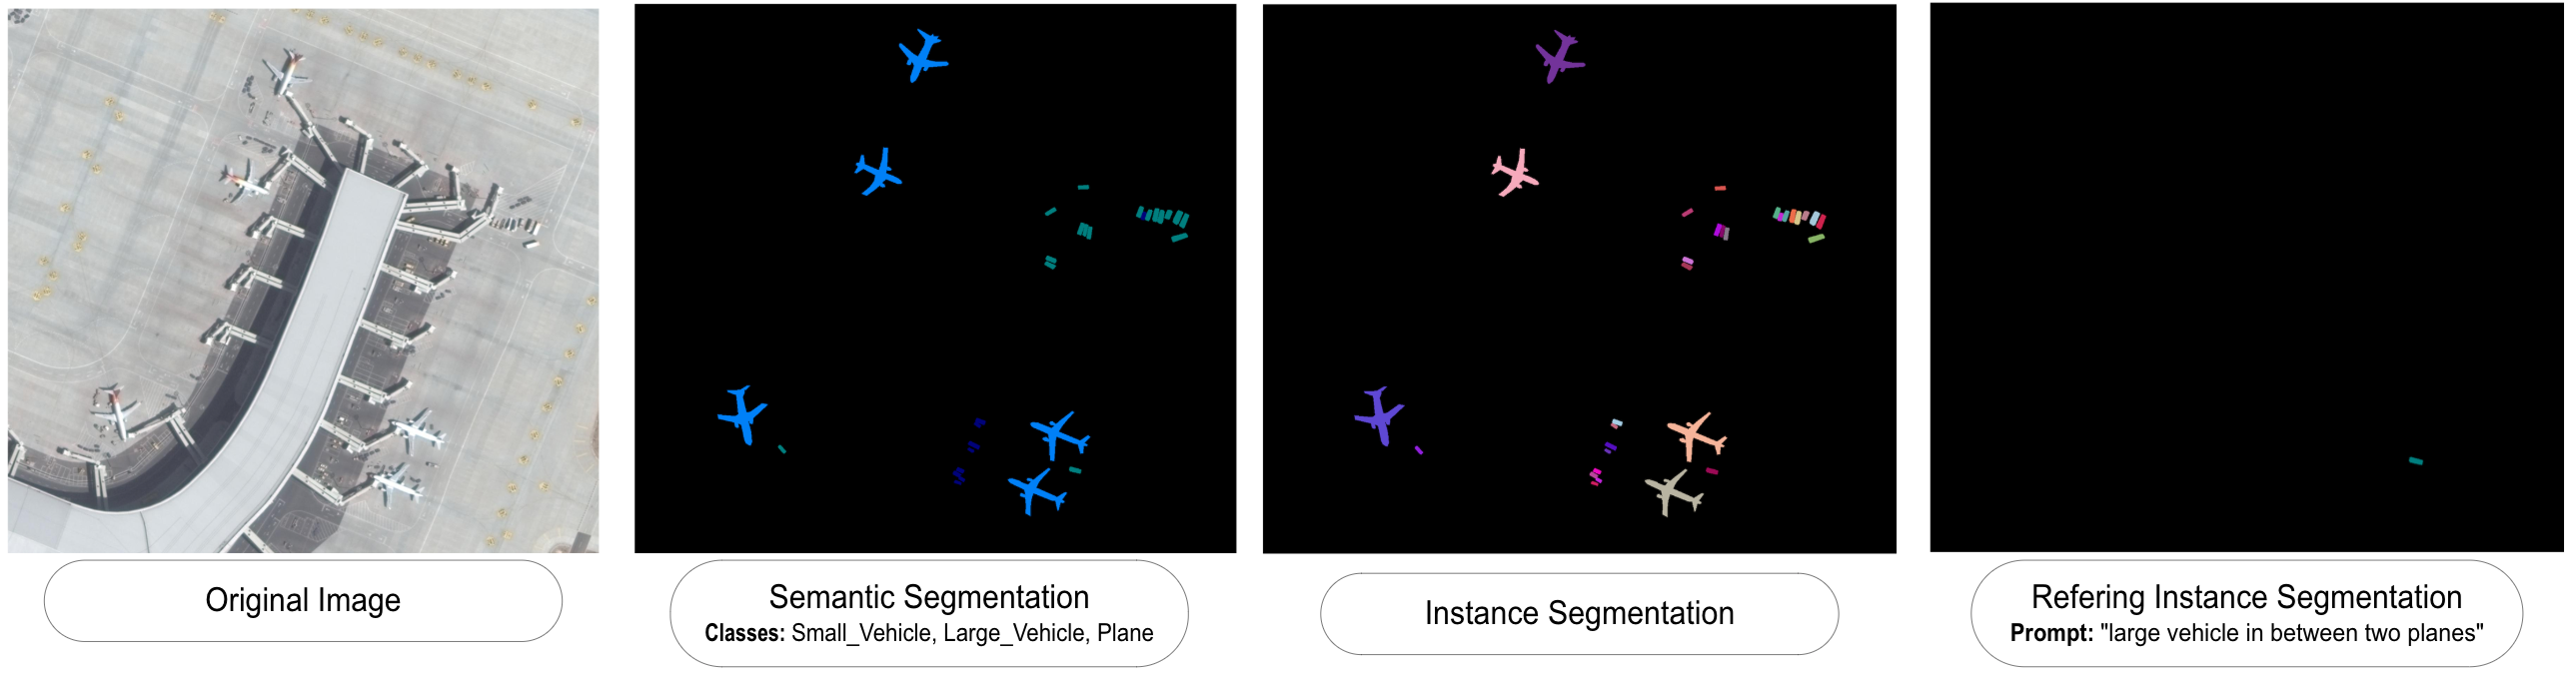
\includegraphics[width=1.0\textwidth]{Images/segmentation.png}
\caption{Comparison of segmentation types: semantic segmentation, instance segmentation, and referring instance segmentation with natural language prompts.}
\label{fig:segmentation}
\end{figure}

% #############################################################################
\section{Vision-Language Models}

Vision-language models represent a significant advancement in multimodal artificial intelligence, enabling systems to understand and reason about both visual and textual information simultaneously. These architectures bridge the gap between computer vision and natural language processing by learning joint representations that capture semantic relationships across modalities.

\subsection{CLIP and Visual-Language Learning}

Contrastive Language-Image Pre-training (CLIP) introduces a powerful framework for learning visual-textual representations through contrastive learning~\cite{clip}. The architecture consists of two separate transformer encoders: an image encoder that processes visual input and a text encoder that handles natural language descriptions, as illustrated in Figure~\ref{fig:clip_architecture}.

The core innovation of CLIP lies in its contrastive pre-training methodology, which learns to align image and text embeddings in a shared representation space. During training, the model processes batches of image-text pairs and computes similarity scores between all possible combinations. For a batch of $N$ image-text pairs, CLIP maximizes the cosine similarity between correct pairs while minimizing similarity between incorrect pairs:

\begin{equation}
\mathcal{L}_{\text{contrastive}} = -\frac{1}{N}\sum_{i=1}^{N} \left[ \log \frac{\exp(\text{sim}(\mathbf{I}_i, \mathbf{T}_i) / \tau)}{\sum_{j=1}^{N} \exp(\text{sim}(\mathbf{I}_i, \mathbf{T}_j) / \tau)} \right],
\end{equation}

where $\mathbf{I}_i$ and $\mathbf{T}_i$ represent image and text embeddings respectively, $\text{sim}(\cdot, \cdot)$ computes cosine similarity, and $\tau$ is a learned temperature parameter that controls the sharpness of the softmax distribution.

This contrastive objective enables CLIP to achieve remarkable zero-shot classification capabilities. Given a new image and a set of candidate class descriptions, the model can classify the image by computing similarities between the image embedding and text embeddings for each class description, selecting the class with the highest similarity score. This approach eliminates the need for task-specific fine-tuning and demonstrates strong generalization across diverse visual domains.

The learned joint embedding space has proven valuable for numerous downstream vision-language tasks beyond classification. The aligned representations enable applications such as image retrieval using text queries, caption generation, visual question answering, and multimodal reasoning tasks. The versatility of CLIP embeddings stems from their ability to capture semantic relationships that transfer across different tasks and domains, making them fundamental building blocks for modern multimodal systems.

\begin{figure}[t]
\centering
\subfigure[Contrastive pre-training methodology.]{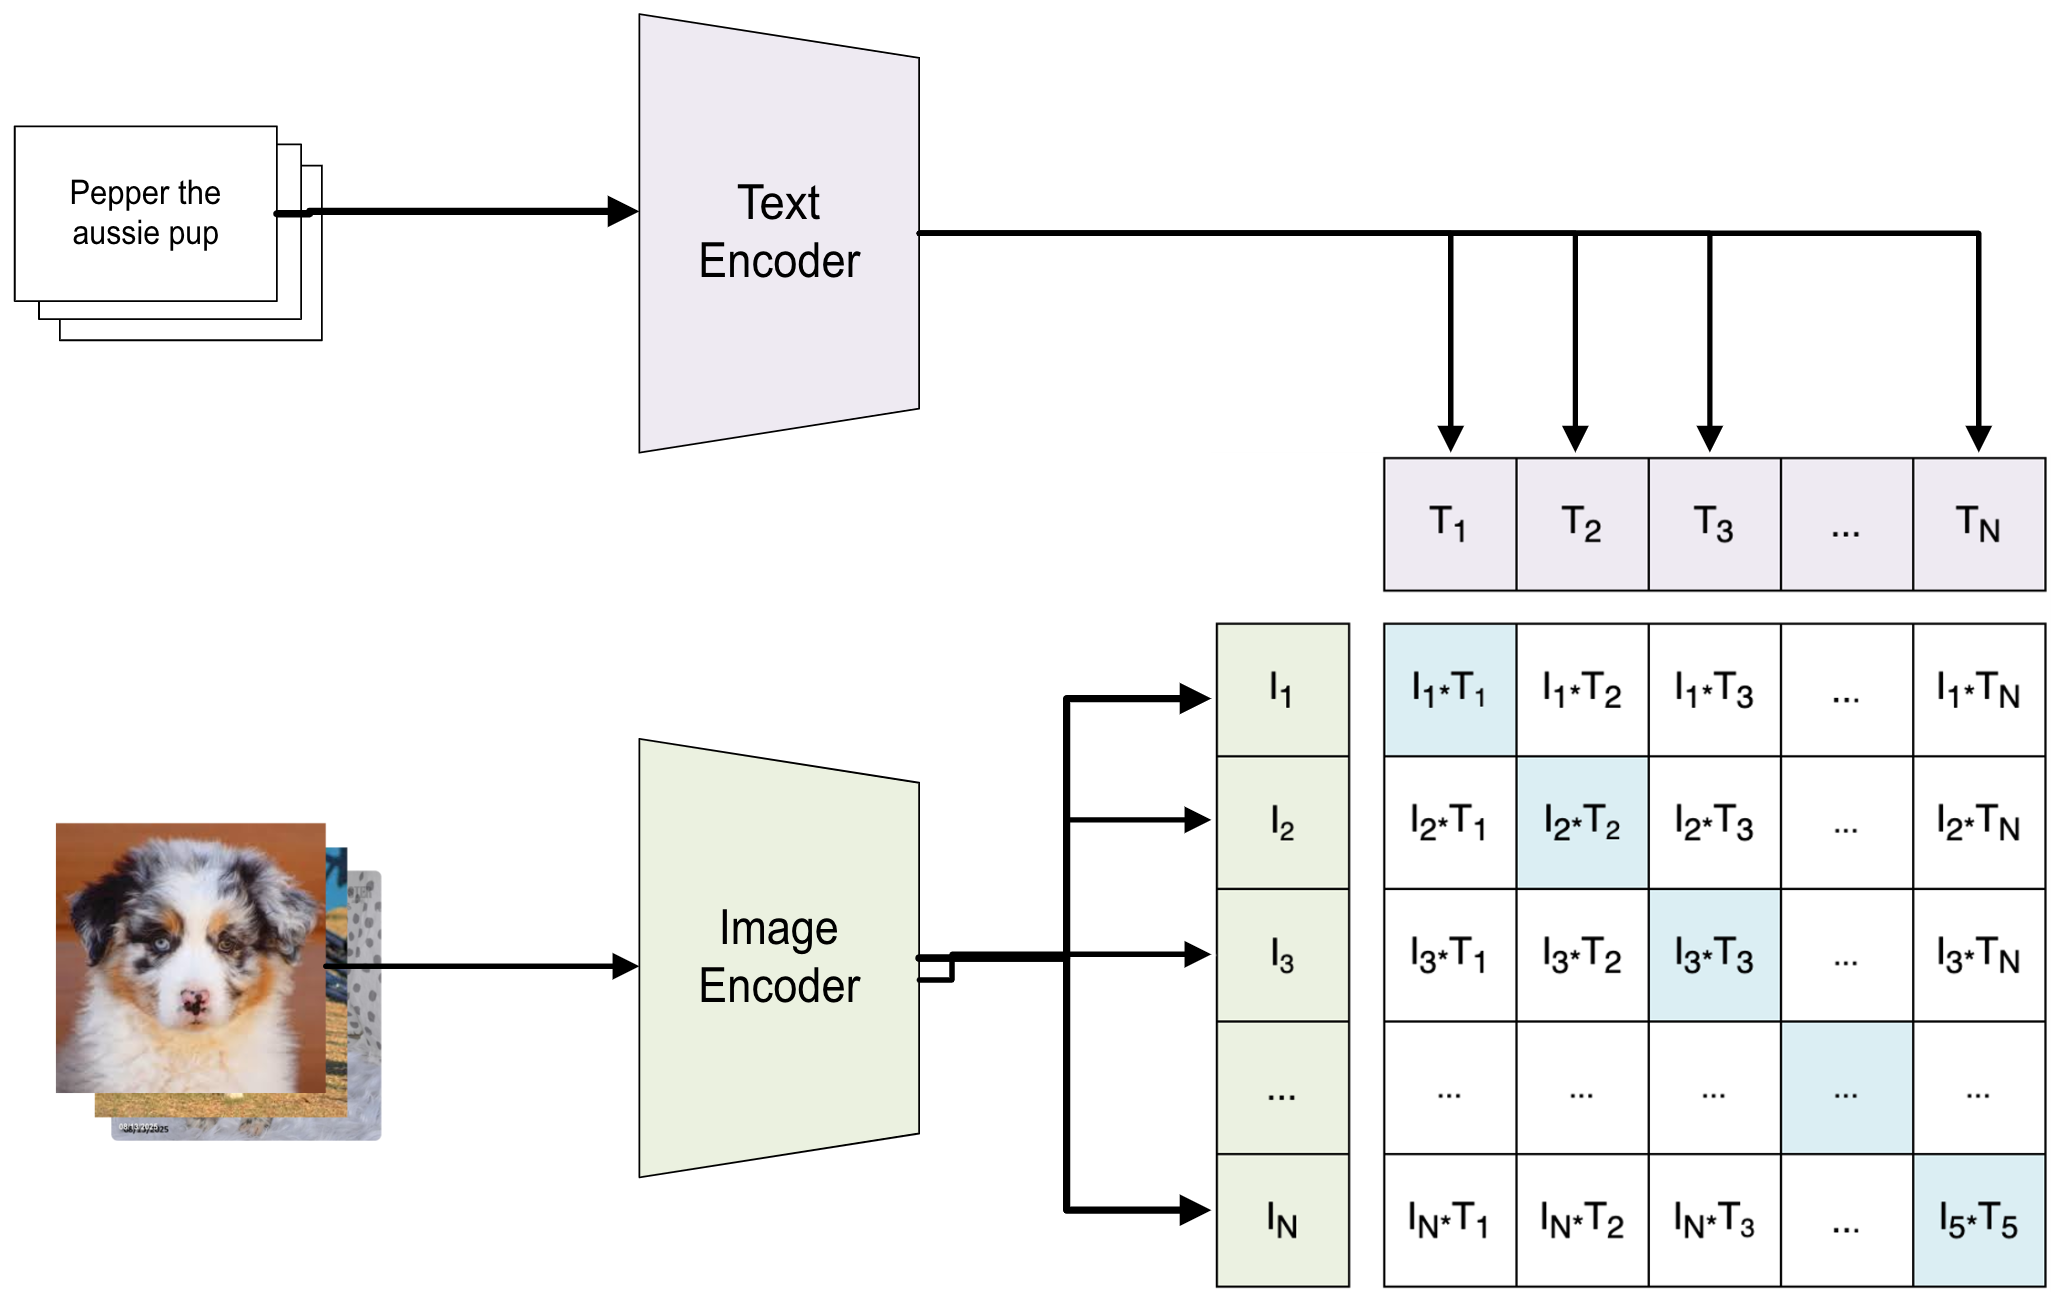
\includegraphics[width=0.45\textwidth]{Images/contrastive_pretraining.png}\label{fig:contrastive_pretraining}}
\hfill
\subfigure[Zero-shot prediction capabilities.]{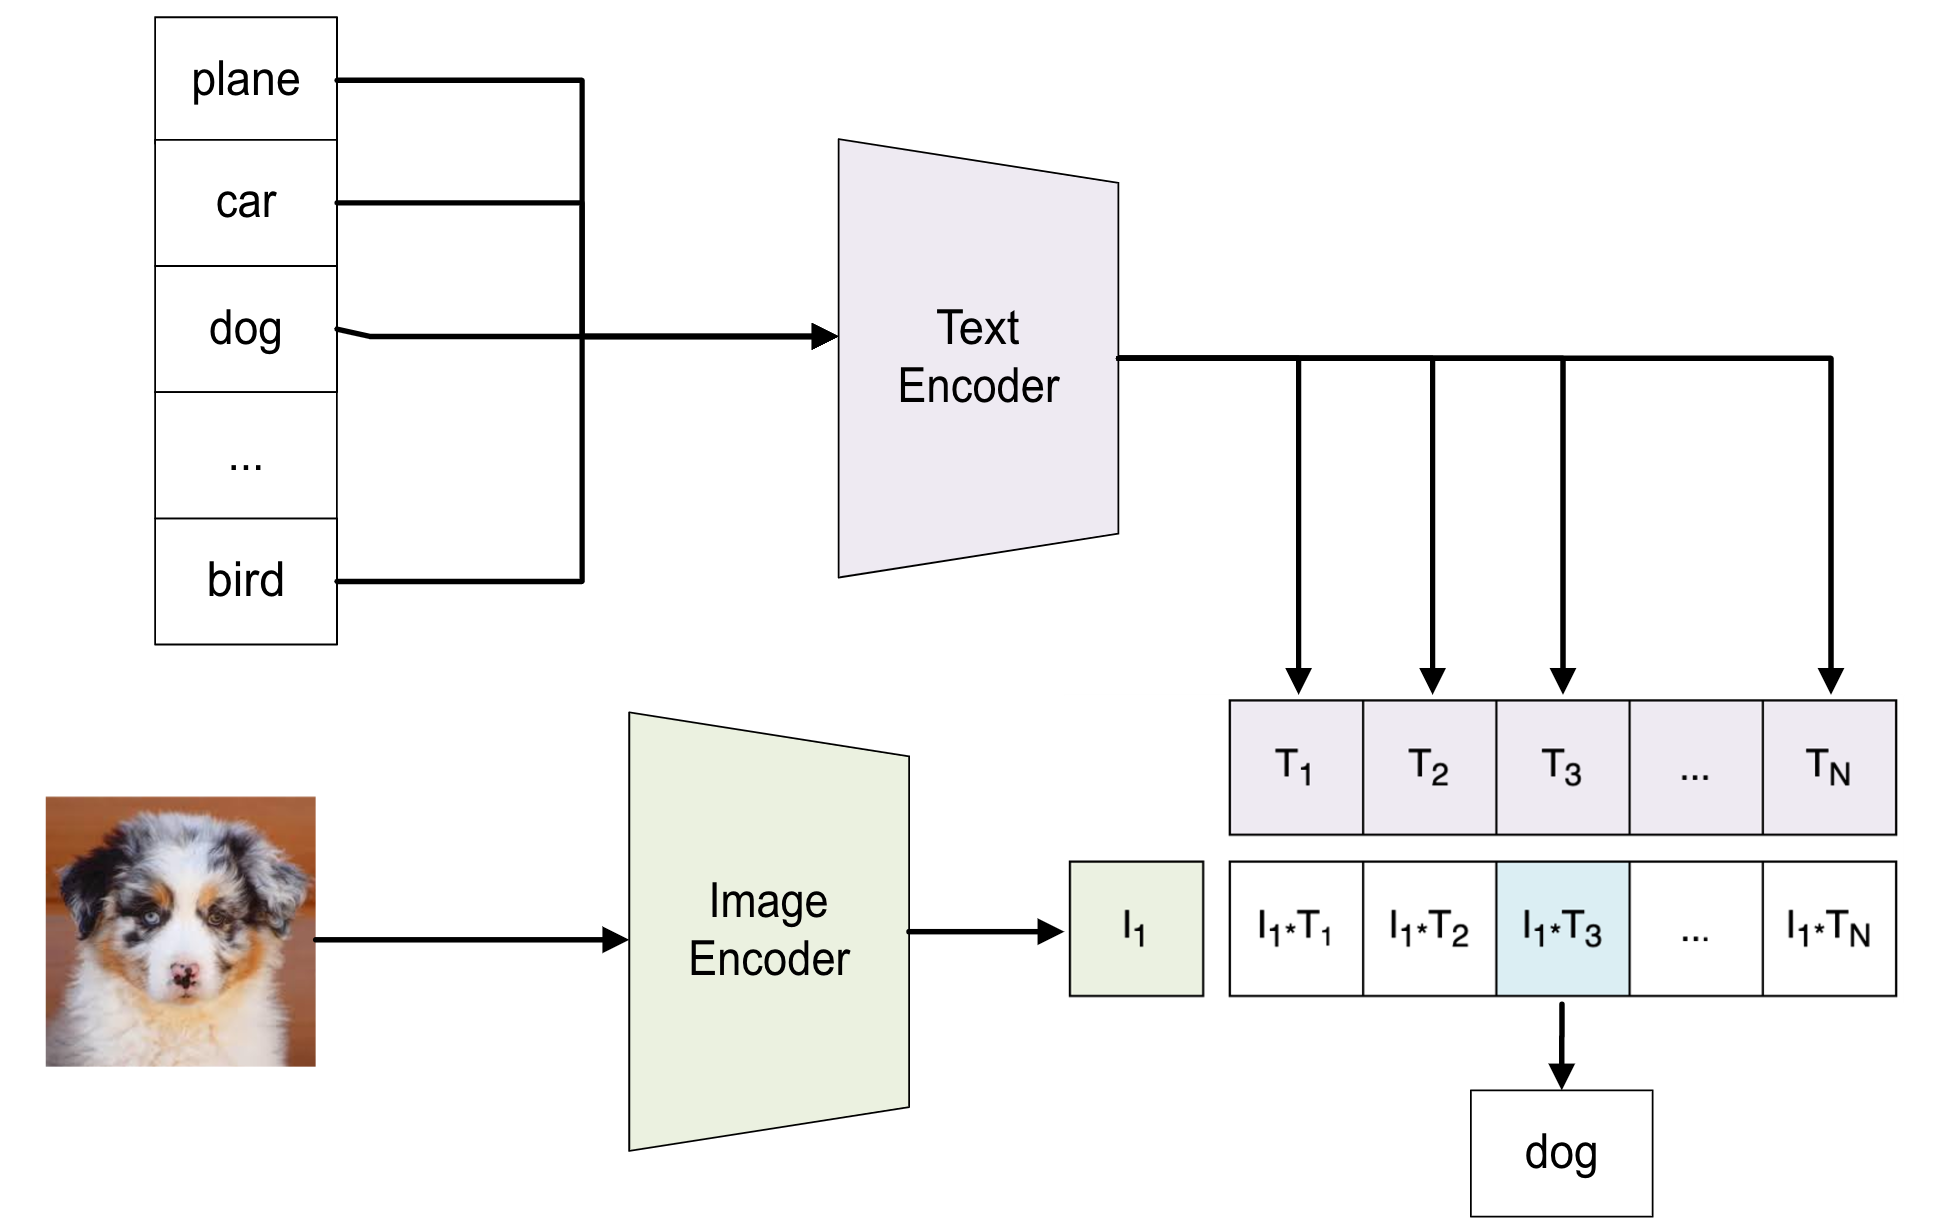
\includegraphics[width=0.45\textwidth]{Images/zero_shot_prediction.png}\label{fig:zero_shot_prediction}}
\caption{CLIP architecture components showing contrastive pre-training and zero-shot prediction mechanisms.}
\label{fig:clip_architecture}
\end{figure}

\subsection{Large Multimodal Language Models}

Large Language Models (LLMs) have emerged as powerful foundation models that demonstrate remarkable capabilities in natural language understanding, generation, and reasoning. These models, exemplified by the GPT (Generative Pre-trained Transformer) family, utilize transformer decoder architectures trained on vast text corpora to learn rich linguistic representations and world knowledge.

The GPT architecture employs a causal transformer decoder that generates text autoregressively, predicting the next token in a sequence based on all previous tokens, as illustrated in Figure~\ref{fig:gpt}. The diagram shows the characteristic feedback mechanism where each predicted token is fed back into the sequence for subsequent predictions. For a sequence of tokens $\mathbf{x} = [x_1, x_2, \ldots, x_t]$, the model processes the entire sequence through multiple transformer layers before computing the probability of the next token $x_{t+1}$ through an output MLP:

\begin{equation}
P(x_{t+1} | x_1, x_2, \ldots, x_t) = \text{softmax}(\mathbf{W}_o \mathbf{h}_t),
\end{equation}

where $\mathbf{h}_t$ represents the hidden state at position $t$ from the final transformer layer and $\mathbf{W}_o$ is the output projection matrix. The training objective maximizes the likelihood of the training sequences:

\begin{equation}
\mathcal{L}_{\text{LM}} = -\sum_{i=1}^{T} \log P(x_i | x_1, \ldots, x_{i-1}),
\end{equation}

where $T$ is the sequence length. This next-token prediction objective, demonstrated in the figure's "Add to sequence" feedback loop, enables LLMs to learn complex linguistic patterns, semantic relationships, and contextual dependencies from large-scale text data.

The versatility of the transformer architecture allows LLMs to process heterogeneous token sequences that extend beyond natural language. In multimodal contexts, the input sequence can include tokens from vision encoders, such as those produced by CLIP's image encoder. Since CLIP's visual representations are aligned with language through contrastive training, LLMs can be trained to understand these visual tokens alongside textual tokens, creating truly multimodal language models. This integration enables the model to process mixed sequences containing both visual and textual information, allowing for sophisticated capabilities such as visual question answering, image captioning with rich contextual descriptions, and instruction-following for complex visual tasks. The extensive world knowledge captured by LLMs during pre-training, combined with their ability to process visual tokens, allows them to provide contextual understanding that goes beyond simple pattern recognition, enabling more nuanced and informative multimodal interactions.

Modern implementations of large multimodal language models demonstrate remarkable capabilities in vision-language understanding and generation~\cite{gemma3,o3,gemini25}.

These systems integrate vision and language to enable multimodal capabilities~\cite{clip,siglip}.

Open-source models integrate vision encoders with transformer decoder architectures, enabling sophisticated multimodal reasoning while maintaining accessibility for research and development~\cite{gemma3,siglip,siglip2}.

Proprietary large-scale models represent the current state-of-the-art in multimodal language modeling, demonstrating advanced capabilities in complex visual reasoning, detailed image analysis, and sophisticated instruction following across multiple domains~\cite{o3}.

For example, OpenAI's o3 family~\cite{o3}.

Similarly, Google's Gemini 2.5~\cite{gemini25}.

These models leverage massive computational resources and extensive multimodal training datasets to achieve performance levels that approach human-level understanding in many vision-language tasks, setting new benchmarks for what is possible in artificial multimodal intelligence.

\begin{figure}[t]
\centering
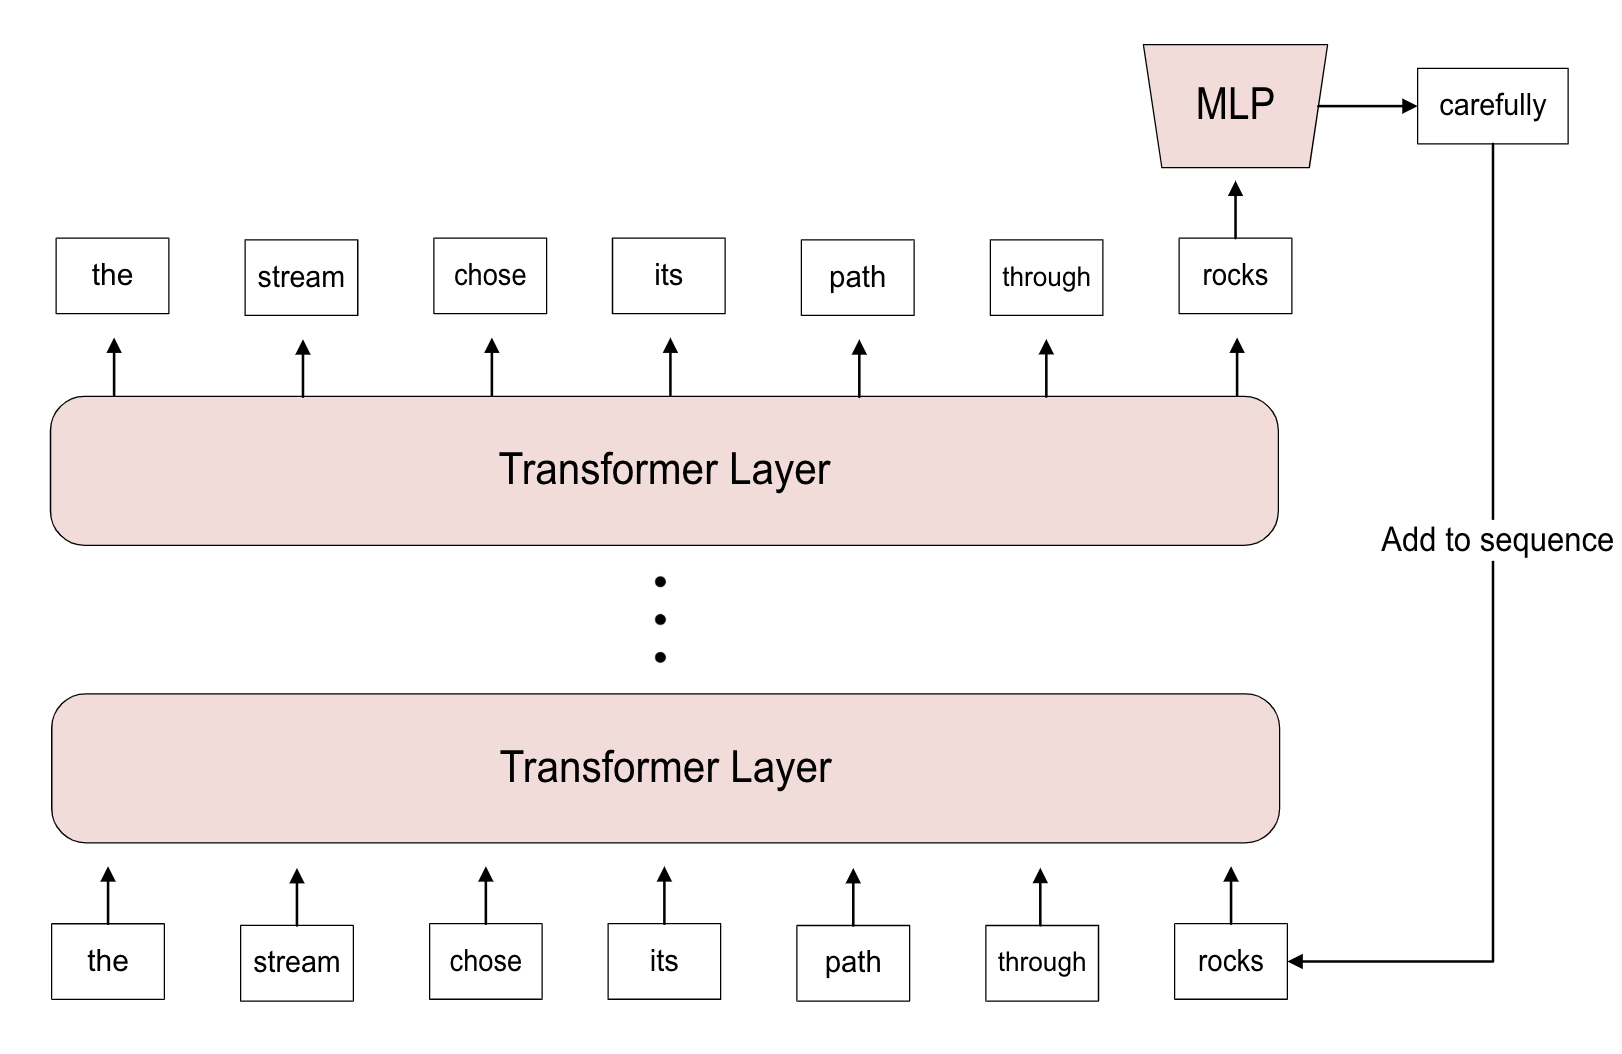
\includegraphics[width=0.8\textwidth]{Images/gpt.png}
\caption{GPT autoregressive language model architecture showing the transformer decoder stack with next-token prediction and feedback mechanism.}
\label{fig:gpt}
\end{figure}

% #############################################################################
\section{Overview}

This chapter has introduced the fundamental technical concepts that underpin modern open-vocabulary referring segmentation systems. Neural networks and deep learning provide the computational foundation through multi-layer perceptrons and gradient-based optimization, enabling the learning of complex patterns from data. The transformer architecture, with its self-attention mechanism, revolutionizes sequence modeling by allowing parallel processing and capturing long-range dependencies across different modalities.

The extension of transformers to computer vision through Vision Transformers demonstrates the versatility of attention mechanisms beyond natural language processing. By treating image patches as sequences, ViTs enable the processing of visual information using the same architectural principles that have proven successful for text, laying the groundwork for unified multimodal architectures.

Image segmentation represents a core computer vision task that partitions images into semantically meaningful regions through dense pixel-level prediction. The progression from semantic segmentation through instance segmentation to referring instance segmentation illustrates the evolution toward more sophisticated scene understanding capabilities that combine visual analysis with natural language comprehension.

Vision-language models, exemplified by CLIP, establish the crucial bridge between visual and textual modalities through contrastive learning approaches. By learning aligned representations across modalities, these models enable zero-shot capabilities and provide the foundation for multimodal understanding. Large multimodal language models further extend this concept by integrating visual tokens into autoregressive generation frameworks, enabling sophisticated reasoning about both textual and visual content.

Together, these fundamental concepts create a comprehensive technical foundation for open-vocabulary referring segmentation systems that can understand natural language descriptions and precisely segment corresponding visual regions in aerial imagery. The following chapters build upon these foundations to examine existing approaches and present novel contributions to this challenging problem domain.